\begin{center}
    \Large{\textbf{Теоретична частина}}    
\end{center}

\vspace{1mm}

Iдеальною оптичною системою називають таку систему, в якiй збергається гомоцентричнiсть пучкiв i
зображень предмета геометрично подiбне до самого предмета. Iдеальна оптична система має вiсь симетрiї,
яку називають головною оптичною вiссю. Променi, що падають на лiнзу паралельно головнiй оптичнiй
осi, сходяться в задньому фокусi системи в просторi зображень (точка $F_2$ на рис.1).Променi,що виходять з
переднього фокуса системи, що знаходяться в просторi предметiв (точка $F_1$ на рис.1) виходять з системи
паралельно до головної оптичної осi. Площина, що проходить через фокус перпендикулярно
до головної оптичної осi, називається фокальною площиною.

\begin{wrapfigure}{r}{0.5\textwidth}    
    \centering
    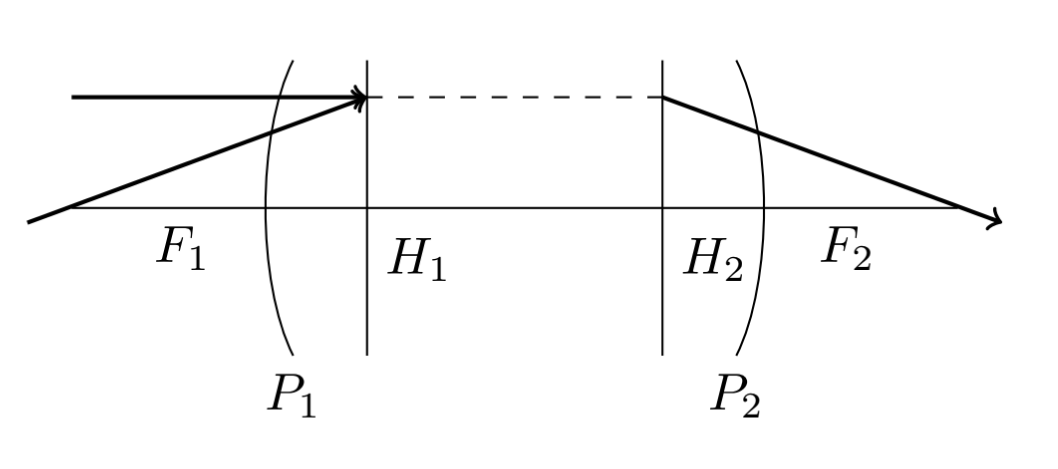
\includegraphics[width=.5\textwidth]{assets/1.png}
    \caption{Хiд променiв у товстiй лiнзi}
\end{wrapfigure}

Розрiзняють також головнi площини ($P_1,P_2$) та головнi точки ($H_1, H_2$)системи. Головна площина перпендикулярна до
головної оптичної осi та проходить через точку перетину фокального променя та паралельного променя. Головнi точки
визначаються к точки перетину головної площини та головної осi. Вiдстанi мiж головними точками та фокусами називають
фокусними вiдстаннями системи: $f_1 = F_1H_1, f2 = F_2H_2$. 
Якщо по обидвi сторони вiд оптичної системи знаходиться одне й теж саме середовище, то $f_1 = f_2 = f$.

Оптичну систему називають збиральною (позитивною), якщо на виходi з неї пучок паралельних променiв
збирається, тобто заднiй фокус розташовано за системою, а переднiй - перед системою вiдносно
напрямку розповсюдження променiв. В цьому випадку фокуснi вiдстанi є позитивними величинами. На
виходi з розсiювальної (вiд’ємної) системи паралельнi променi розходяться, заднiй фокус розташовано 
перед системою, а переднiй — за системою, фокуснi вiдстанi вважаються вiд’ємними. Вiдстань до об’єкта g 
та до зображення b звичайно вiдраховують вiд вiдповiдних головних площин ($P_1, P_2$,вiдповiдно). 
Цi величини вважаються позитивними, якщо об’єкт знаходиться перед головною площиною в просторi об’єктiв,
а зображення — за головною площиною в просторi зображень.

Зауважимо, що головнi площини можуть знаходитись як в межах оптичною системи, так i ззовнi. В
межах геометричної оптики можна вивести просте спiввiдношення мiж величинами $g, b$ та $f$: уваги змiну
фаз свiтлової хвилi пiд час вiдбиття вiд гранцi подiлу скло-повiтря,коли показник заломлення першого
середовища бiльше за показник заломлення другого, та пiд час ввiдбиття вiд гранцi повiтря-скло, коли
навпаки показник заломлення першого середовища меньше за показник заломлення другого. Вiдомо, що
для електричного вектора у першому випадку вiдбиття вiдбувається без змiни фаз, а в другому призводить
до змiни фаз на $\pi$, фаза магнiтного вектора, навпаки,змiнюється на $\pi$ тiльки пiд час першого вiдбиття.
Таким чином, променi 1 i 2 набувають рiзницi фаз $\pi$, що вiдповiдає додатковiй рiзницi ходу $\frac{\lambda}{2}$, а повна
рiзниця ходу:

\begin{equation} \label{eq:1}
    g^{-1} + b^{-1} = f^{-1}
\end{equation}


\begin{figure}{h}
    \centering    
    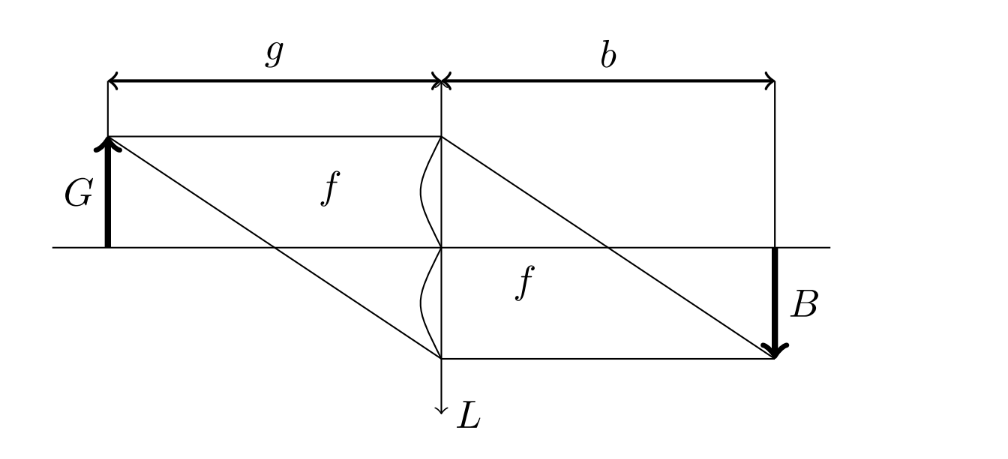
\includegraphics[width=.6\textwidth]{assets/2.png}       
    \caption{Побудова геометричного зображення вiд тонкої збиральної лiнзи}
\end{figure}

На практицi найчастiше застосовуються тонкi лiнзи, геометричрнi розмiри якх в напрямку головної
оптичної осi значно меншi за фокусну вiдстань. Для тонкої лiнзи передня та задня головнi площини
спiвпадають i знаходяться приблизно в центрi лiнзи. Розглянемо рис.2. На ньому побудовано зображення
об’єкта вiд тонкої збиральної лiнзи. З геометричних мiркувань очевидно, що коефiцiєнт збiльшення
лiнзи V.

\begin{equation} \label{eq:2}
    V = \frac{B}{G} = \frac{b}{g} = \frac{b-f}{f} 
\end{equation}

За допомогою спiввiдношення \ref{eq:2} можна переписати формулу \ref{eq:1}
через вiдстанi вiд об’єкта до вiдповiдних фокусiв:

\begin{equation} \label{eq:3}
    (b-f)(g-f) = f^2
\end{equation}